\section{definitive assembly reference}



\lstset{language=myasm}

\section{definitive sources}
\begin{frame}{x86-64 assembly}
\begin{itemize}
\item history: AMD constructed 64-bit extension to x86 first
    \begin{itemize}
    \item marketing term: AMD64
    \end{itemize}
\item Intel first tried a new ISA (Itanium), which failed
\item Then Intel copied AMD64
    \begin{itemize}
    \item marketing term: EM64T
        \begin{itemize}\item Extended Memory 64 Technology\end{itemize}
    \item later marketing term: Intel 64
    \end{itemize}
\item both Intel and AMD have manuals --- definitive reference
\end{itemize}
\end{frame}

\begin{frame}
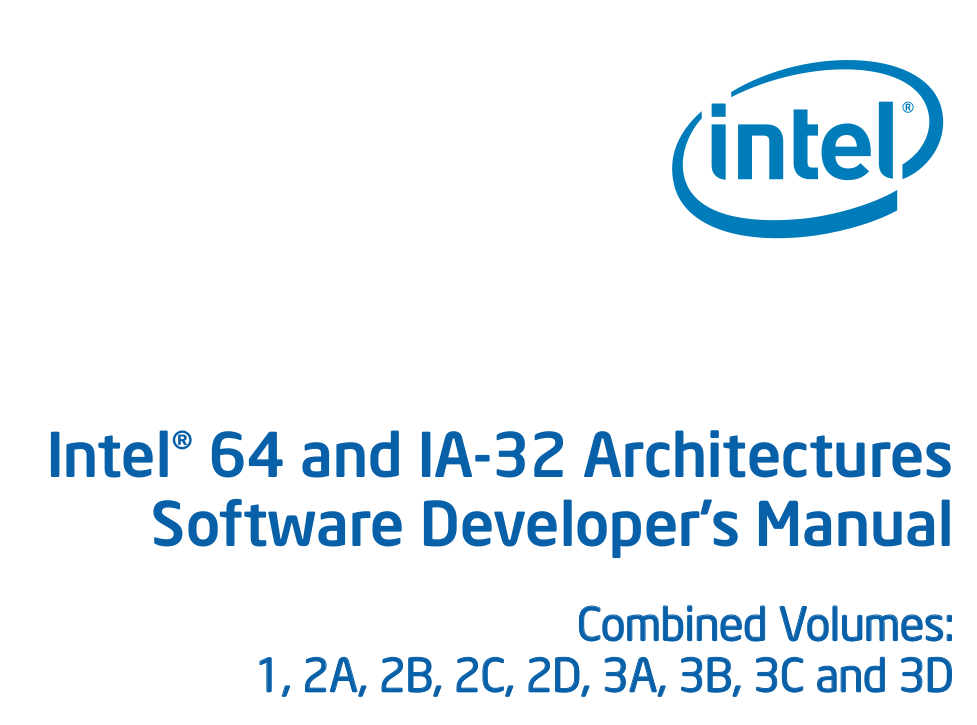
\includegraphics[height=0.9\textheight]{../asm/manual-screenshot}
\end{frame}

\begin{frame}{x86-64 manuals}
\begin{itemize}
\item Intel manuals:
    \begin{itemize}
    \item \small \url{https://software.intel.com/en-us/articles/intel-sdm}
    \item 24 MB, 4684 pages
    \item Volume 2: instruction set reference (2190 pages)
    \end{itemize}
\item AMD manuals:
    \begin{itemize}
    \item \small \url{https://support.amd.com/en-us/search/tech-docs}
    \item ``AMD64 Architecture Programmer's Manual''
    \end{itemize}
\end{itemize}
\end{frame}

\begin{frame}{example manual page}
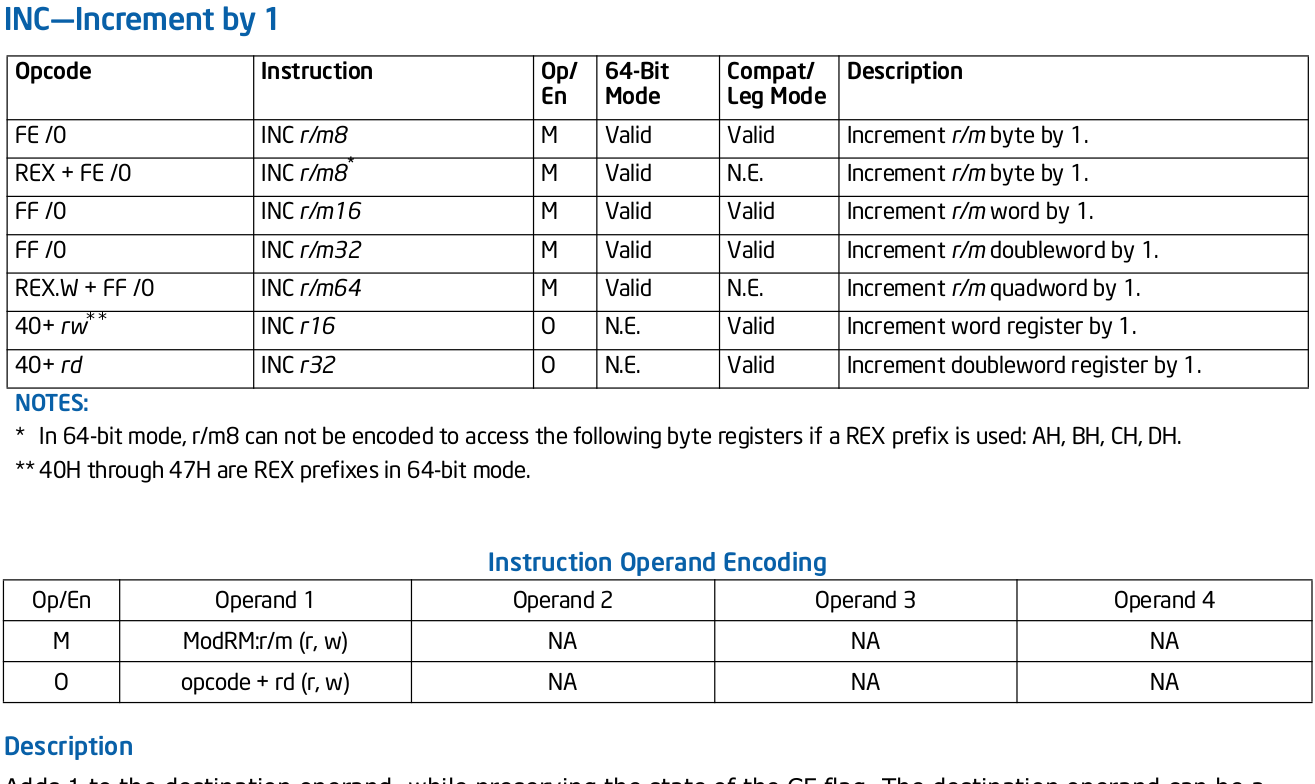
\includegraphics[width=\textwidth]{../asm/example-manual}
\end{frame}

\begin{frame}{instruction listing parts (1)}
    \begin{itemize}
    \item opcode --- first part of instruction encoding
        \begin{itemize}
        \item yes, variable length
        \item ``REX''???
        \item more later (today or next week)
        \end{itemize}
    \item instruction --- Intel assembly skeleton
    \item {\tt r/m32} --- 32-bit memory or register value
    \item 64-bit mode --- does instruction exist in 64-bit mode?
    \item compat/leg mode --- in 16-bit/32-bit modes?
    \end{itemize}
\end{frame}

\begin{frame}{instruction listing parts (2)}
    \begin{itemize}
    \item dscription + operation (later on page)
        \begin{itemize}
        \item text and pseudocode description
        \end{itemize}
    \item flags affected
        \begin{itemize}
        \item flags --- used by {\tt jne}, etc.
        \end{itemize}
    \item exceptions --- how can OS be called from this?
        \begin{itemize}
        \item example: can invalid memory access happen?
        \end{itemize}
    \end{itemize}
\end{frame}


\section{registers and overlap}

\usetikzlibrary{calc}

\begin{frame}{recall: x86-64 general purpose registers}
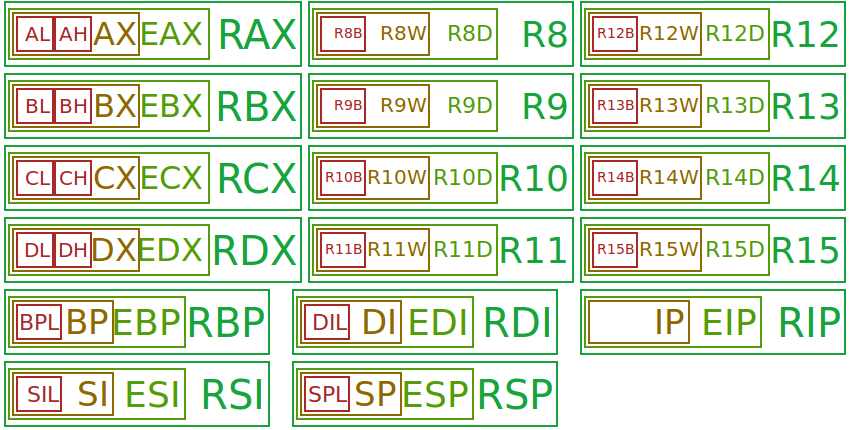
\includegraphics[width=\textwidth]{../asm/x86-gprs}
\imagecredit{Immae via Wikipedia}
\end{frame}

\begin{frame}[fragile,label=overlap]{overlapping registers (1)}
\begin{itemize}
\item setting 32-bit registers sets \myemph{whole} 64-bit register
\item extra bits are always zeroes
\end{itemize}
\begin{lstlisting}[style=small]
movq $0x123456789abcdef, %rax
xor %eax, %eax
// %rax is 0, not 0x1234567800000000
movl $-1, %ebx
// %rbx is 0xFFFFFFFF, not -1 (0xFFFFF...FFF)
\end{lstlisting}
\end{frame}

\begin{frame}[fragile,label=overlap2]{overlapping registers (2)}
\begin{itemize}
\item setting \myemph{8/16-bit registers} doesn't change rest of 64-bit register:
\end{itemize}
\begin{lstlisting}[style=small]
movq $0x12345789abcdef, %rax
movw $0xaaaa, %ax
// %rax is 0x123456789abaaaa
\end{lstlisting}
\end{frame}



\section{Intel v ATT syntax}


\begin{frame}{AT\&T versus Intel syntax}
    \begin{itemize}
    \item AT\&T syntax: \\ {\tt movq \$42, 100(\%rbx,\%rcx,4)}
    \item Intel syntax: \\ {\tt mov QWORD PTR [rbx+rcx*4+100], 42}
    \item effect (pseudo-C): \\ {\tt memory[rbx + rcx * 4 + 100] <- 42}
    \end{itemize}
\end{frame}

\begin{frame}[fragile,label=att1]{AT\&T syntax (1)}
\begin{lstlisting}
movq $42, 100(%rbx,%rcx,4)
\end{lstlisting}
    \begin{itemize}
    \item destination \myemph{last}
    \item constants start with {\tt \$}
    \item registers start with {\tt \%}
    \end{itemize}
\end{frame}

\begin{frame}[fragile,label=att2]{AT\&T syntax (2)}
\begin{lstlisting}
movq $42, 100(%rbx,%rcx,4)
\end{lstlisting}
    \begin{itemize}
    \item operand length: {\tt q}
        \begin{itemize}
        \item {\tt l} = 4; {\tt w} = 2; {\tt b} = 1
        \item can be omitted when implied by context
        \end{itemize}
    \item {\tt 100(\%rbx,\%rcx,4)}: \\ {\tt memory[100 + rbx + rcx * 4]}
    \item {\tt sub \%rax, \%rbx}: {\tt rbx $\leftarrow$ rbx - rax}
    \end{itemize}
\end{frame}

\begin{frame}{Intel syntax}
    \begin{itemize}
    \item destination \myemph{first}
    \item {\tt [...]} indicates location in memory
    \item {\tt QWORD PTR [...]} for 8 bytes in memory
        \begin{itemize}
        \item DWORD for 4
        \item WORD for 2
        \item BYTE for 1
        \item can be omitted when implied by context
        \end{itemize}
    \end{itemize}
\end{frame}




\section{LEA}


% FIXME: move this?
\begin{frame}[fragile,label=LEA]{On LEA}
    \begin{itemize}
    \item LEA = Load Effective Address
    \item uses the syntax of a memory access, but\ldots{}
    \item just computes the address and uses it:
    \item {}\lstinline|leaq 4(%rax), %rax| same as \lstinline|addq $4, %rax|
        \begin{itemize}
        \item almost --- doesn't set condition codes
        \end{itemize}
    \end{itemize}
\end{frame}

\begin{frame}[fragile,label=LEATricks]{LEA tricks}
    \begin{itemize}
    \item {}\lstinline|leaq (%rax,%rax,4), %rax| multiplies {\tt \%rax} by 5
        \begin{itemize}
        \item {\tt address-of(memory[rax + rax * 4])}
        \end{itemize}
    \item {}\lstinline|leal (%rbx,%rcx), %eax| adds rbx + rcx into eax
        \begin{itemize}
        \item ignores top 64-bits
        \end{itemize}
    \end{itemize}
\end{frame}
 % FIXME: move to backup?

\section{exercise (lea + mov)}

\begin{frame}[fragile,label=question]{question}
\lstset{style=small,language=myasm,deletekeywords=bl}
\begin{lstlisting}
.data
string:
    .asciz "abcdefgh"
.text
    movq $string, %rax
    movq string, %rdx
    movb (%rax), %bl
    leal 1(%rbx), %ebx
    movb %bl, (%rax)
    movq %rdx, 4(%rax)
\end{lstlisting}
{\small What is the final value of string?}
\begin{tabular}{ll}
a. \texttt{"abcdabcd"} & d. \texttt{"abcdefgh"} \\
b. \texttt{"bbcdefgh"} & e. something else / not enough info \\
c. \texttt{"bbcdabcd"} & ~ \\
\end{tabular}
\end{frame}


\section{objdump output}
\newcommand{\varMark}[2]{\myemph<#1>{#2}}
\newcommand{\varOnly}[2]{\only<#1>{#2}}

\begin{frame}[fragile,label=disassemblyRead]{reading objdump disassembly}
\begin{itemize}
\item often, we'll want to work from binaries to assembly
\item tool we'll use on Linux: \texttt{objdump}
\item example from \textit{\tt objdump --disassemble} of hello-world program:
\end{itemize}
\begin{Verbatim}[fontsize=\fontsize{10}{11},commandchars=\\\{\}]
\varMark{2}{0000000000001060 <main>}:
  \varMark{3}{1060}:  \varMark{4}{f3 0f 1e fa}           endbr64 
  \varMark{3}{1064}:  \varMark{4}{50}                    push   %rax
  \varMark{3}{1065}:  \varMark{4}{48 8d 3d 98 0f 00 00}  lea    \varMark{6}{0xf98(%rip)},%rdi \varMark{6}{# 2004 <_IO_stdin_used+0x4>}
          \varOnly{6}{\myemph{# 2004 <_IO_stdin_used+0x4>}}
  \varMark{3}{106c}:  \varMark{4}{e8 df ff ff ff}        \varMark{5}{callq  1050 <puts@plt>}
  \varMark{3}{1071}:  \varMark{4}{31 c0}                 xor    %eax,%eax
  \varMark{3}{1073}:  \varMark{4}{5a}                    pop    %rdx
  \varMark{3}{1074}:  \varMark{4}{c3}                    retq   
\end{Verbatim}
\begin{tikzpicture}[overlay,remember picture]
\tikzset{
    note/.style={
        draw=red,very thick,fill=white,at={([yshift=-1cm]current page.north)},anchor=north,
        align=left
    }
}
\begin{visibleenv}<2>
    \node[note] {symbol main at address 0x1060};
\end{visibleenv}
\begin{visibleenv}<3>
    \node[note] {
        first column: instruction addresses in hexadecimal \\
        (if executable/library has fixed address, \\
        actual addresses they'll be loaded to)
    };
\end{visibleenv}
\begin{visibleenv}<4>
    \node[note] {
        machine code as list of byte values in hexadecimal
    };
\end{visibleenv}
\begin{visibleenv}<5>
    \node[note] {
        \verb|callq 1050 <puts@plt>| \\
        call to address 0x1050 \\
        and \texttt{puts@plt} is at that address
    };
\end{visibleenv}
\begin{visibleenv}<6>
    \node[note] {
        \verb|lea 0xf98(%rip),%rdi # 2004 <_IO_stdin_used+0x4>| \\
        \verb|0xf98(%rip)| computes address 0x2004 \\
        which is \texttt{0x4} bytes after \verb|_IO_stdin_used|
    };
\end{visibleenv}
\end{tikzpicture}
\end{frame}


\section{Linux x86-64 calling conventions}

\usetikzlibrary{arrows.meta,calc,matrix}

\begin{frame}{Linux x86-64 calling convention}
    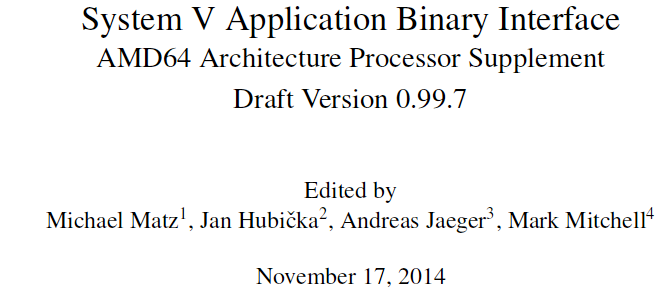
\includegraphics[width=\textwidth]{../asm/sysv-abi-front}
\end{frame}

\begin{frame}{Linux x86-64 calling summary}
\begin{itemize}
    \item first 6 arguments: \%rdi, \%rsi, \%rdx, \%rcx, \%r8, \%r9
        \begin{itemize}
        \item floating point arguments: \%xmm0, \%xmm1, etc.
        \end{itemize}
    \item additional arguments: push on stack
    \item return address: push on stack
        \begin{itemize}
        \item {\tt call}, {\tt ret} instructions assume this
        \end{itemize}
    \item return value: \%rax
\end{itemize}
\end{frame}



\begin{frame}[fragile,label=conventionEx]{calling convention example}
\begin{lstlisting}[language=C,style=small]
int foo(int a, int b, int c, int d, int e, int f, int g, int h);
...
foo(1, 2, 3, 4, 5, 6, 7, 8);
\end{lstlisting}
\begin{lstlisting}[language=myasm,style=small]
pushq   $8
pushq   $7
movl    $6, %r9d
movl    $5, %r8d
movl    $4, %ecx
movl    $3, %edx
movl    $2, %esi
movl    $1, %edi
call    foo
/* return value in %eax */
\end{lstlisting}
\end{frame}

 % FIXME: note location of definitive reference, move to backup


\begin{frame}[fragile,label=callStack]{the call stack}
\begin{lstlisting}[language=C,style=small]
foo(a,b,c,d,e,f,g,h);
\end{lstlisting}
\begin{tikzpicture}
\tikzset{>=Latex}
\matrix[tight matrix,nodes={text width=7cm,font=\tt}] (theStack) {
    \ldots \\
    \normalfont (stack allocations in caller) \\
    \normalfont (saved registers, if any) \\
    h \\
    g \\
    \normalfont return address \\
    \normalfont (first stack allocation in {\tt foo}) \\
    \ldots \\
};
\draw[very thick,->] ([xshift=0.25cm]theStack-1-1.east)  -- ([xshift=0.25cm]theStack-8-1.east)
    node[right] {decreasing addresses};
\draw[red,thick,->] (theStack-6-1.east) -- ++(.5cm,0cm) node[right] {stack pointer after call};
\end{tikzpicture}
\end{frame}


\section{floating point}

% FIXME: examples with C code

\usetikzlibrary{calc}

\begin{frame}{floating point operations}
    \begin{itemize}
    \item x86 has two ways to do floating point
    \item method one --- legacy: x87 floating point instructions
        \begin{itemize}
        \item still common in 32-bit x86
        \end{itemize}
    \item method two --- SSE instructions
        \begin{itemize}
        \item work more like what you expect
        \end{itemize}
    \end{itemize}
\end{frame}

\begin{frame}[fragile,label=x87Stack]{x87 floating point stack}
    \begin{itemize}
    \item x87: 8 floating point registers
        \begin{itemize}
        \item {\tt \%st(0)} through {\tt \%st(7)}
        \end{itemize}
    \item arranged as a \myemph{stack of registers}
    \item example: \lstinline|fld 0(%rbx)| 
        \begin{tabular}{l@{: }ll}
        ~ & before & after \\
        {\tt st(0)} & 5.0 & (value from memory at {\tt \%rbx}) \\
        {\tt st(1)} & 6.0 & 5.0 \\
        {\tt st(1)} & 7.0 & 6.0 \\
        \ldots      & \ldots & \ldots \\
        {\tt st(6)} & 10.0 & 9.0 \\
        {\tt st(7)} & 11.0 & 10.0 \\
        \end{tabular}
    \end{itemize}
\end{frame}

\begin{frame}{x87}
    \begin{itemize}
    \item not going to talk about x87 more in this course
    \item essentially obsolete with 64-bit x86
    \end{itemize}
\end{frame}

\begin{frame}[fragile,label=sseRegs]{SSE registers}
    \begin{itemize}
    \item SSE and SSE2 extensions brought \myemph{vector instructions}
    \end{itemize}
\lstset{
    language=myasm,
    style=small,
    moredelim={**[is][\btHL<2|handout:0>]{&2}{&}},
    moredelim={**[is][\btHL<3|handout:0>]{&3}{&}},
    moredelim={**[is][\btHL<4|handout:0>]{&4}{&}},
    morekeywords={.float,movps,addps},
}
\begin{lstlisting}
&2numbers: .float 1 .float 2 .float 3. float 4&
ones:    .float 1 .float 3 .float 5 .float 7
result:  .float 0 .float 0 .float 0 .float 0
...
&3movps& numbers, %xmm0
movps ones, %xmm1
&4addps& %xmm1, %xmm0
movps %xmm0, result
/* result contains: 1+1=2,2+3=5,3+5=8,4+7=11 */
\end{lstlisting}
\begin{tikzpicture}[overlay,remember picture]
    \coordinate (overlayPlace) at ([xshift=1cm,yshift=.5cm]current page.center);
    \tikzset{overThing/.style={
        draw=red,very thick,rectangle,at=(overlayPlace),
        anchor=west,align=left,fill=white,
    }}
    \begin{visibleenv}<2|handout:0>
        \node [overThing] {array of 4 floats};
    \end{visibleenv}
    \begin{visibleenv}<3|handout:0>
        \node [overThing] {move packed single \\ (single-precision float)};
    \end{visibleenv}
    \begin{visibleenv}<4|handout:0>
        \node [overThing] {add packed single \\ (single-precision float)};
    \end{visibleenv}
\end{tikzpicture}
\end{frame}

\begin{frame}{XMM registers}
\begin{itemize}
\item {\tt \%xmm0} through {\tt \%xmm15} {\small ({\tt \%xmm8} on 32-bit)}
\item each holds 128-bits ---
    \begin{itemize}
    \item 32-bit floating point values ({\tt addps}, etc.)
    \item 64-bit floating point values ({\tt addpd}, etc.) 
    \item 64/32/16/8-bit integers ({\tt paddq/d/w/b}, etc.)
    \item \myemph<2>{a 32-bit floating point value}, 96 unused bits ({\tt addss}, {\tt movss}, etc.)
    \item \myemph<2>{a 64-bit floating point value}, 64 unused bits ({\tt addsd}, {\tt movsd}, etc.)
    \end{itemize}
\vspace{.5cm}
\item more recently: {\tt \%ymm0} through {\tt \%ymm15} (256-bit, ``AVX'')
    \begin{itemize}
    \item overlap with {\tt\%xmm{\it X}} registers
    \end{itemize}
\end{itemize}
\end{frame}

\begin{frame}[fragile,label=fpExample]{FP example}
\lstset{language=myasm,morekeywords={movss,mulss,subq}}
\begin{lstlisting}
multiplyEachElementOfArray:
/* %rsi = array, %rdi length,
   %xmm0 multiplier */
loop:   test %rdi, %rdi
        je done
        movss (%rsi), %xmm1
        mulss %xmm0, %xmm1
        movss %xmm1, (%rsi)
        subq $1, %rdi
        addq $4, %rsi
        jmp loop
done:   ret
\end{lstlisting}
\end{frame}




\section{addressing modes} % FIXME: move to backup?


\begin{frame}[fragile,label=addressing1]{addressing modes (1)}
    \begin{itemize}
        \item {\small AT\&T} {\tt \%reg}\\ {\small Intel} {\tt REG}
        \item {\small AT\&T} {\tt \$constant} \\{\small Intel} {\tt constant}
        \item {\small AT\&T} {\tt displacement(\%base, \%index, scale)} \\
        {\small Intel} {\tt [base+index*scale+displacement]}
            \begin{itemize}
            \item {\tt displacement} (absolute)
            \item {\tt displacement(\%base)}
            \item {\tt displacement(,\%index, scale)}
            \end{itemize}
    \end{itemize}
\end{frame}

\begin{frame}[fragile,label=addressing2]{addressing modes (2)}
    \begin{itemize}
        \item {\small AT\&T} {\tt displacement(\%rip)} \\
              {\small Intel} {\tt [RIP + displacement]}
            \begin{itemize}
            \item value in memory displacement bytes after current instruction
            \end{itemize}

\begin{lstlisting}
thing: .quad 42
...
movq thing(%rip), %rax
\end{lstlisting}
        \begin{itemize}
        \item Linux assembler: thing(\%rip) another way of referencing thing
            \begin{itemize}
            \item thing at 0x2000, instr ends at 0x3000 $\rightarrow$ same as \texttt{movq -0x1000(\%rip), \%rax}
            \item other assemblers may have quite different syntax for this
            \end{itemize}
        \item encoded as offset from \myemph{address of next instruction}
        \item (normally: label encoded as 32 or 64-bit address)
        \item helps \myemph{relocatable code}
        \end{itemize}
    \end{itemize}
\end{frame}

\begin{frame}[fragile,label=addressing3]{addressing modes (3)}
    \begin{itemize}
        \item {\small AT\&T} {\tt jmp *\%rax} \\
            {\small Intel} {\tt jmp RAX}
        \begin{itemize}
        \item jmp to address specified by RAX
        \end{itemize}
    \item {\small AT\&T} {\tt jmp *(\%rax)} \\
        {\small Intel} {\tt jmp [RAX]}
        \begin{itemize}
        \item read value from memory at RAX
        \item PC becomes location in that value
        \end{itemize}
    \item {\small AT\&T} {\tt jmp *(\%rax,\%rbx,8)} \\
        {\small Intel} {\tt jmp [RAX+RBX*8]}
    \end{itemize}
\end{frame}




\subsection{where is jump exericse}
\begin{frame}[fragile,label=whereIsJumpEx]{where is the jump?}
\begin{Verbatim}
0xA0000: lea 0x1234(%rip), %rax  # 0xA123b
    (Intel syntax: LEA RAX, [RIP + 0x1234])
0xA0007: add %rbx, %rax
    (Intel syntax: ADD RAX, RBX)
0xA000A: jmp *(%rax)
    (Intel syntax: JMP [RAX])
...
0xA123B: 0x30000 (64-bit value)
....
0xB123B: 0x40000 (64-bit-value)
...
0xB124B: 0x50000 (64-bit value)
\end{Verbatim}
If \%rax initially contains 0x40, then the instruction
executed after the jump is at address \rule{1cm}{1pt}.
\end{frame}


% FIXME: question on what jmp jumps to

\section{endbr64}

\begin{frame}[fragile,label=endbr64]{ENDBR64?}
partial output of \textit{objdump --disassemble}:
\begin{Verbatim}[fontsize=\small]
0000000000001060 <main>:
    1060:       f3 0f 1e fa             endbr64 
    1064:       50                      push   %rax
    1065:       48 8d 3d 98 0f 00 00    lea    0xf98(%rip),%rdi        # 2004 <_IO_stdin_used+0x4>
    106c:       e8 df ff ff ff          callq  1050 <puts@plt>
    1071:       31 c0                   xor    %eax,%eax
    1073:       5a                      pop    %rdx
    1074:       c3                      retq   
\end{Verbatim}
\hrule
\begin{itemize}
\item endbr64: (currently) nop instruction that marks destination of branches
\item why? --- we'll explain (much) later
\end{itemize}
\end{frame}


\section{segmentation}
% FIXME: example of thread-local storage?
\usetikzlibrary{arrows.meta,calc,matrix,positioning,shapes.multipart}

\begin{frame}[fragile,label=vm]{recall(?): virtual memory}
\begin{itemize}
\item illuision of \myemph{dedicated memory}
\end{itemize}
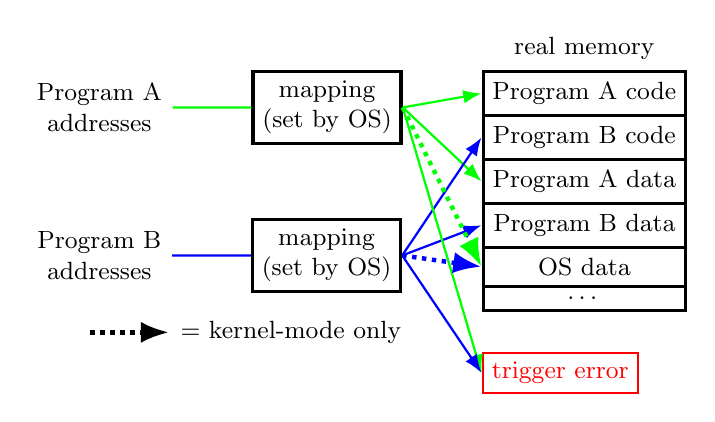
\begin{tikzpicture}
\tikzset{
    every node/.style={font=\small},
}
\node[align=center] (progAAddr) {Program A \\ addresses};
\node[below=1cm of progAAddr,align=center] (progBAddr) {Program B \\ addresses};
\node[draw, right=1cm of progAAddr,align=center] (translationA) { mapping \\ (set by OS) };
\node[draw, right=1cm of progBAddr,align=center] (translationB) { mapping \\ (set by OS) };
\node[draw,rectangle split, rectangle split parts=6, anchor=north west,label={north:real memory}] (mem) at ([xshift=1cm]translationA.north east) {
    \nodepart{one}
    Program A code 
    \nodepart{two}
    Program B code
    \nodepart{three}
    Program A data
    \nodepart{four}
    Program B data
    \nodepart{five}
    OS data
    \nodepart{six}
    \ldots
};
\draw[-Latex,green,thick] (progAAddr) -- (translationA) (translationA.east) -- (mem.one west);
\draw[-Latex,green,thick] (translationA.east) -- (mem.three west);
\draw[-Latex,blue,thick] (progBAddr) -- (translationB) (translationB.east) -- (mem.two west);
\draw[-Latex,blue,thick] (translationB.east) -- (mem.four west);
\node[thick,red,draw,anchor=north west] (error) at ([yshift=-.5cm]mem.south west) {trigger error};
\draw[-Latex,green,thick] (translationA.east) -- (error.west);
\draw[-Latex,blue,thick] (translationB.east) -- (error.west);
\draw[-Latex,green,ultra thick,dotted] (translationA.east) -- (mem.five west);
\draw[-Latex,blue,ultra thick,dotted] (translationB.east) -- (mem.five west);
\draw[-Latex,ultra thick,dotted] ([xshift=-3cm,yshift=-.5cm]translationB.south) -- ([xshift=-2cm,yshift=-.5cm]translationB.south)
    node[right] {= kernel-mode only};
\end{tikzpicture}
\end{frame}


\begin{frame}[fragile,label=segmentation]{segmentation}
    \begin{itemize}
    \item before virtual memory, there was \myemph{segmentation}
    \end{itemize}
\begin{tikzpicture}
    \tikzset{>=Latex}
    \node[draw,label={north:address},rectangle split,rectangle split parts=2,
        rectangle split horizontal,font=\small,align=left] (address) {
        segment \#: \\ \color{orange!70!black}{\tt 0x1} \nodepart{two} offset: \\ \color{magenta!70!black}{\tt 0x23456}
    };
    \matrix[tight matrix,nodes={text width=2cm,font=\small\tt,text depth=.4ex,text height=1.2ex},
        column 1/.style={nodes={text width=1.5cm}},
        anchor=north west,
        visible on=<1>,
    ] (table) at ([xshift=.5cm]address.north east){
        seg \# \& base \& limit \\
        0 \& 0x14300 \& 0x60000 \\
        |[orange!70!black]| 1 \& |[blue!70!black]| 0x50000 \& |[green!70!black]| 0x6F000 \\
        2 \& 0x70000 \& 0x30000 \\
    };
    \matrix[tight matrix,nodes={text width=2cm,font=\small\tt,text depth=.4ex,text height=1.2ex},
        column 1/.style={nodes={text width=1.5cm}},
        column 3/.style={nodes={font=\scriptsize\tt, text width=6cm}},
        anchor=north west,
        visible on=<2>,
    ] (table2) at ([xshift=.5cm]address.north east){
        seg \# \& base \& limit \\
        0 \& 0x0 \& 0xFFFF FFFF FFFF FFFF \\
        |[orange!70!black]| 1 \& |[blue!70!black]| 0x0 \& |[green!70!black]| 0xFFFF FFFF FFFF FFFF \\
        2 \& 0x0 \& 0xFFFF FFFF FFFF FFFF \\
    };
    \node[draw,circle,font=\large] (plus) at ([yshift=-2cm]address.two south) { $+$ };
    \node[font=\large,draw] (less) at (table-3-3.south |- plus) { $<=$ };
    \draw[magenta!70!black,thick,->] (address.two south) -- (plus);
    \draw[blue!70!black,thick,->] (table-3-2.south) |- (plus);
    \draw[green!70!black,thick,->] ([xshift=.25cm]table-3-3.south) -- ([xshift=.25cm]less.north);
    \draw[magenta!70!black,thick,->] (address.two south) -- ($(plus.north) + (0, .5cm)$) -| ([xshift=-.25cm]less.north);
    \draw[thick,->] (plus) -- ++ (0,-1cm) node[below] { computed address };
    \draw[thick,->] (less) -- ++ (0,-1cm) node[below,align=center] { no segmentation \\ fault?};
\end{tikzpicture}
\end{frame}


\begin{frame}[fragile, label=x86Seg]{x86 segmentation}
\begin{itemize}
\item addresses you've seen are the \myemph{offsets}
\item but every access uses a segment number!
\item segment numbers come from registers
    \begin{itemize}
    \item CS --- code segment number (jump, call, etc.)
    \item SS --- stack segment number (push, pop, etc.)
    \item DS --- data segment number (mov, add, etc.)
    \item ES --- addt'l data segment (string instructions)
    \item FS, GS --- extra segments (never default)
    \end{itemize}
\item instructions can have a \myemph{segment override}:
\begin{lstlisting}
movq $42, %fs:100(%rsi)
    // move 42 to segment (# in FS),
    // offset 100 + RSI 
\end{lstlisting}
\end{itemize}
\end{frame}

\begin{frame}[fragile,label=x86SegPic]
\vspace{-.25cm}
\tikzset{every picture/.style={very thick},every node/.style={fill=white,inner sep=.1mm}}
\begin{tikzpicture}
\node[anchor=north west] at (0,0){
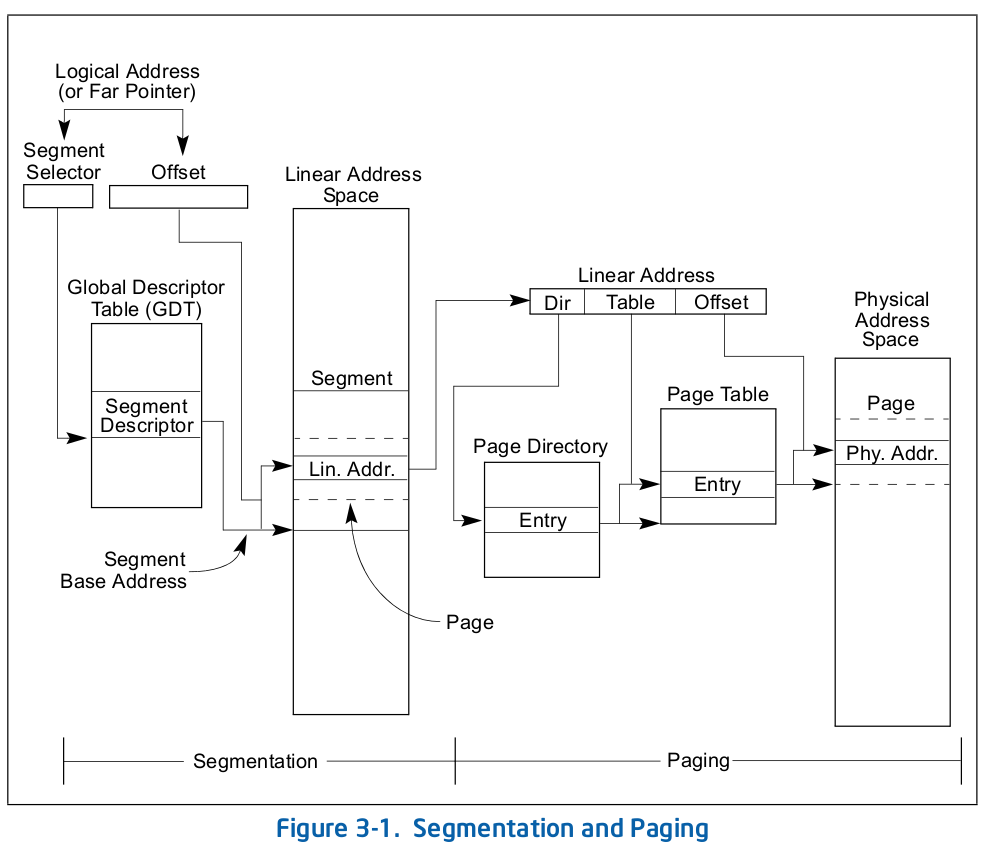
\includegraphics[width=0.78\textwidth]{../asm/seg-and-page}
};
%\draw[help lines] (0,0) grid (12, -8);
\begin{visibleenv}<2>
    \draw[blue] (0.8,-0.8) rectangle (2.5,-1.4);
    \node[text=blue!70!black,anchor=south,font=\small] at (1.6,-.8) {program address};
    \draw[green] (6.4,-3.3) rectangle (9.1,-3.9);
    \node[text=green!70!black,anchor=south,font=\small,align=center] at (7.5,-3.3) {after segmentation \\
                                                  ``virtual address''};
    \draw[magenta] (0.9,-3.4) rectangle (2.8,-6.1);
    \node[text=magenta!70!black,anchor=south,font=\small] at (1.8,-3.4) {segment table};
\end{visibleenv}
\begin{visibleenv}<3>
    \draw[red] (0.3,-1.6) rectangle (1.4,-2.4);
    \node[text=red,anchor=west] at (1.4,-2.0) {from instruction + segment register};
\end{visibleenv}
\end{tikzpicture}
\imagecredit{Figure: Intel manuals, Vol 3A}
\end{frame}

\begin{frame}{x86 segment descriptor}
\vspace{-.25cm}
\tikzset{every picture/.style={very thick},every node/.style={fill=white,inner sep=.2mm}}
\begin{tikzpicture}
\node[anchor=north west] at (0,0){
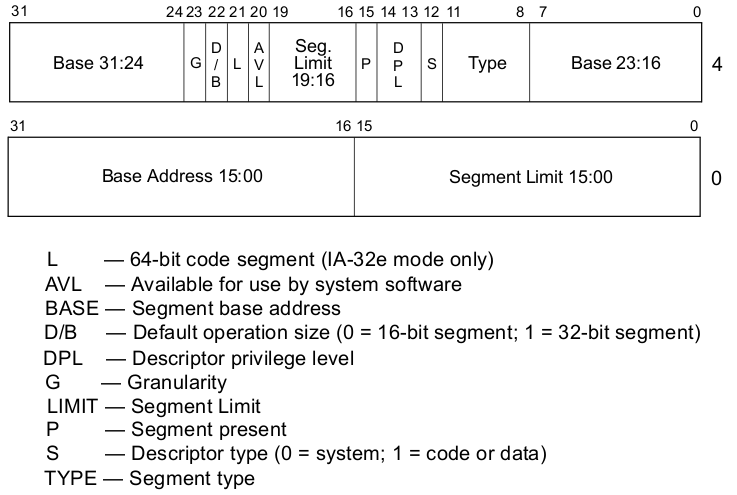
\includegraphics[width=0.78\textwidth]{../asm/segment-descr}
};
%\draw[help lines] (0,0) grid (12, -8);
\begin{visibleenv}<2>
\draw[draw=red] (0.6, -5.4) rectangle (5.8, -5.8) node[right,text=red] {
    user or kernel mode? (if code)
};
\end{visibleenv}
\begin{visibleenv}<3>
\draw[draw=red] (0.6, -3.9) rectangle (8.0, -4.3);
\draw[draw=red] (0.6, -5.0) rectangle (11.0, -5.4);
\node[draw=red,text=red!60!black,anchor=north] at (5.0, -5.6) {
    64-bit or 32-bit or 16-bit mode? (if code)
};
\end{visibleenv}
\end{tikzpicture}
\imagecredit{Figure: Intel manuals, Volume 3A}
\end{frame}


\begin{frame}{64-bit segmentation}
\begin{itemize}
\item in 64-bit mode:
\item limits are ignored
\item base addresses are ignored
\item \ldots except for {\tt \%fs}, {\tt \%gs}
    \begin{itemize}
    \item when explicit segment override is used
    \end{itemize}
\item effectively: extra pointer register
\end{itemize}
\end{frame}




\subsection{thread-local storage example}
\begin{frame}{thread-local storage}
    \begin{itemize}
    \item Linux, Windows use \%fs, \%gs for thread-local storage
    \vspace{.5cm}
    \item variables that have different values in each thread
    \item e.g. for program using multiple cores \\ 
          to track different values for each core
    \end{itemize}
\end{frame}

\begin{frame}[fragile,label=tlsExample1]{TLS example (read) (C)}
\begin{lstlisting}[language=C]
#include <threads.h>
thread_local int thread_local_value = 0;
int get_thread_local() {
    return thread_local_value;
}
\end{lstlisting}
\hrule
\begin{Verbatim}[fontsize=\small]
0000000000001149 <get_thread_local>:
    1149:       f3 0f 1e fa             
                    endbr64 
    114d:       64 8b 04 25 fc ff ff ff
                    mov    %fs:0xfffffffffffffffc,%eax
    1155:       c3  
                    retq   
\end{Verbatim}
\hrule
\begin{Verbatim}[fontsize=\fontsize{9}{10}\selectfont]
TLS off    0x0000000000002df0 vaddr 0x0000000000003df0 paddr 0x0000000000003df0 align 2**2
    filesz 0x0000000000000000 memsz 0x0000000000000004 flags r--
\end{Verbatim}
\end{frame}

\begin{frame}[fragile,label=tlsExample2]{TLS example (write) (C)}
\begin{lstlisting}[language=C]
#include <threads.h>
thread_local int thread_local_value = 0;
void set_thread_local(int new_value) {
    thread_local_value = new_value;
}
\end{lstlisting}
\hrule
\begin{Verbatim}[fontsize=\fontsize{10}{11}\selectfont]
0000000000001156 <set_thread_local>:
    1156:       f3 0f 1e fa 
                    endbr64 
    115a:       64 89 3c 25 fc ff ff ff
                    mov    %edi,%fs:0xfffffffffffffffc
    1162:       c3
                    retq
\end{Verbatim}
\end{frame}



